% =====================================================================
%  CAPÍTULO 3 -- MODELAGEM DA SOLUÇÃO
%  (Regulamento, Art. 9º, item iii)
% ---------------------------------------------------------------------
%  Três "olhares" complementares:
%   - FUNCIONAL: O QUE o sistema faz para cada usuário (casos de uso);
%   - ESTÁTICO:  DE QUE o sistema é feito (modelo de dados);
%   - DINÂMICO:  COMO o sistema se comporta ao longo do tempo.
%  Os diagramas deste capítulo são desenhados em TikZ, direto no LaTeX.
% =====================================================================

\chapter{Modelagem funcional, estática e dinâmica}
\label{cap:modelagem}

O RoundUp é composto por um aplicativo móvel, usado pelos três perfis, e
por serviços gerenciados do Firebase: autenticação (Firebase
Authentication), banco de dados de documentos (Cloud Firestore),
armazenamento de arquivos (Cloud Storage) e funções executadas no servidor
(Cloud Functions). As regras de acesso aos dados ficam nas regras de
segurança do Firestore, e as regras de gamificação (pontos, níveis,
sequência e medalhas) são aplicadas a partir dos registros de presença
validados.

\section{Modelagem funcional}
\label{sec:modelagem-funcional}

O sistema possui três atores. O \textbf{aluno} registra presença e
acompanha a própria evolução. O \textbf{professor} gerencia turmas,
sessões, presenças, missões e graduações. A \textbf{academia} pode fazer
tudo o que o professor faz e, além disso, gerencia os professores
vinculados a ela e consulta uma visão consolidada. Por isso, nos
diagramas de casos de uso, a academia aparece como especialização do
professor: ela herda os casos de uso de gestão e acrescenta os seus. Essa
generalização foi uma correção feita durante o projeto, que antes tratava
apenas dois atores, e se refletiu em todos os artefatos seguintes:
requisitos, modelo de dados, regras de segurança e protótipo de telas,
cujas visões de professor e academia compartilham a mesma estrutura de
``gestor''.

Os requisitos funcionais originaram 30 casos de uso (UC01 a UC30),
organizados nas mesmas sete categorias da base de requisitos. A
\autoref{fig:casos-uso} mostra a visão geral, com os pacotes e os atores
que participam de cada um, e as figuras seguintes detalham os casos de
uso de cada pacote. Os diagramas foram modelados em PlantUML, e o código
de cada um acompanha o projeto.

\begin{figure}[!htb]
  \centering
  \caption{Visão geral dos casos de uso do RoundUp, por pacote}
  \label{fig:casos-uso}
  \begin{tikzpicture}[
      font=\scriptsize,
      pac/.style={draw, minimum width=3.6cm, minimum height=0.75cm, align=center, fill=black!5},
      ator/.style={align=center},
      lig/.style={thin},
      ger/.style={-{Triangle[open,length=2.5mm,width=2.5mm]}, thin}]
    \node[draw, rounded corners=2pt, minimum width=5.2cm, minimum height=8.6cm] (sis) at (0,0) {};
    \node[anchor=north west] at (sis.north west) {\textbf{RoundUp}};
    \node[pac] (con) at (0, 3.1) {Contas (UC01--UC05)};
    \node[pac] (vin) at (0, 2.0) {Vínculos (UC06--UC08)};
    \node[pac] (ges) at (0, 0.9) {Gestão (UC20--UC25)};
    \node[pac] (tre) at (0,-0.2) {Treinos (UC09--UC15)};
    \node[pac] (cnf) at (0,-1.3) {Conformidade (UC26--UC28)};
    \node[pac] (ret) at (0,-2.4) {Retenção (UC29--UC30)};
    \node[pac] (gam) at (0,-3.5) {Gamificação (UC16--UC19)};
    \node[ator] (al) at (-5.2,-0.3) {\Large$\bigcirc$\\[-1pt]\textbf{Aluno}};
    \node[ator] (pr) at (5.2,-0.9) {\Large$\bigcirc$\\[-1pt]\textbf{Professor}};
    \node[ator] (ac) at (5.2, 2.7) {\Large$\bigcirc$\\[-1pt]\textbf{Academia}};
    \foreach \p in {con,vin,tre,cnf,ret,gam} \draw[lig] (al.east) -- (\p.west);
    \foreach \p in {con,vin,ges,tre,cnf,ret} \draw[lig] (pr.west) -- (\p.east);
    \foreach \p in {con,vin,ges} \draw[lig] (ac.west) -- (\p.east);
    \draw[ger] (ac.south) -- (pr.north);
  \end{tikzpicture}
  \fonte{Elaborado pelo autor (2026). A academia herda os pacotes do
         professor; as linhas da academia indicam os pacotes com casos de
         uso exclusivos dela.}
\end{figure}

\begin{figure}[!htb]
  \centering
  \caption{Casos de uso do pacote Contas}
  \label{fig:uc-contas}
  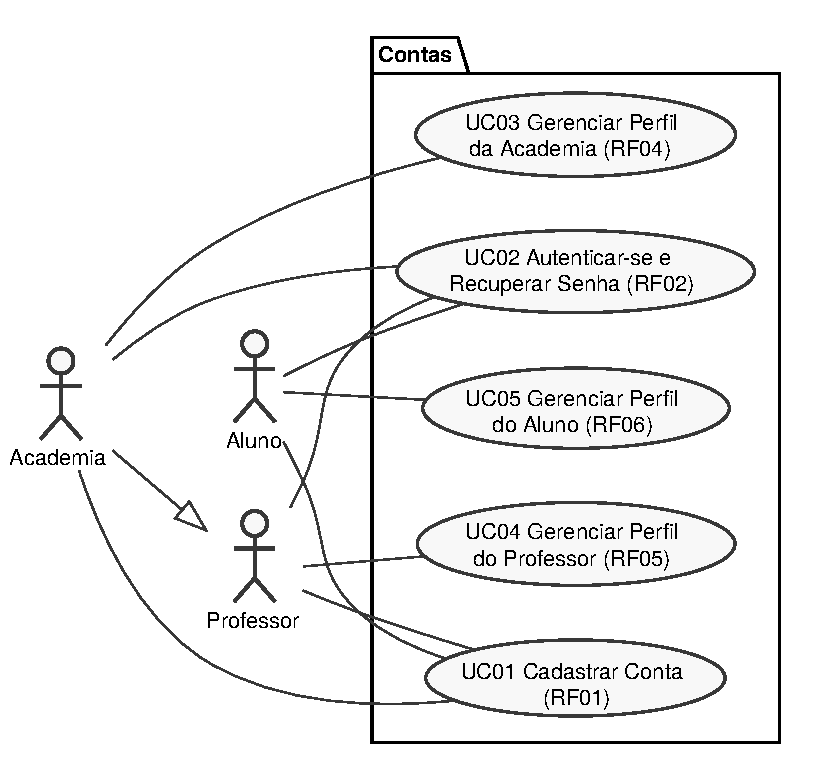
\includegraphics[width=0.62\textwidth]{figuras/uc-1-contas.pdf}
  \fonte{Elaborado pelo autor (2026).}
\end{figure}

\begin{figure}[!htb]
  \centering
  \caption{Casos de uso do pacote Vínculos}
  \label{fig:uc-vinculos}
  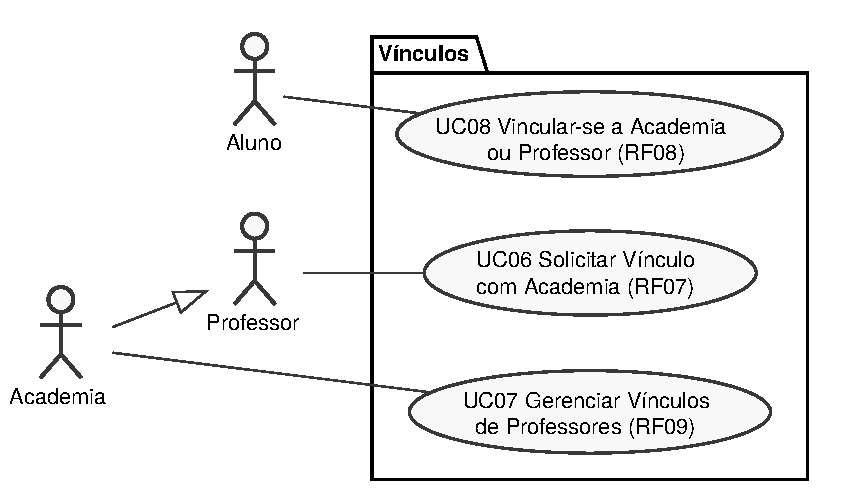
\includegraphics[width=0.62\textwidth]{figuras/uc-2-vinculos.pdf}
  \fonte{Elaborado pelo autor (2026).}
\end{figure}

\begin{figure}[!htb]
  \centering
  \caption{Casos de uso do pacote Treinos}
  \label{fig:uc-treinos}
  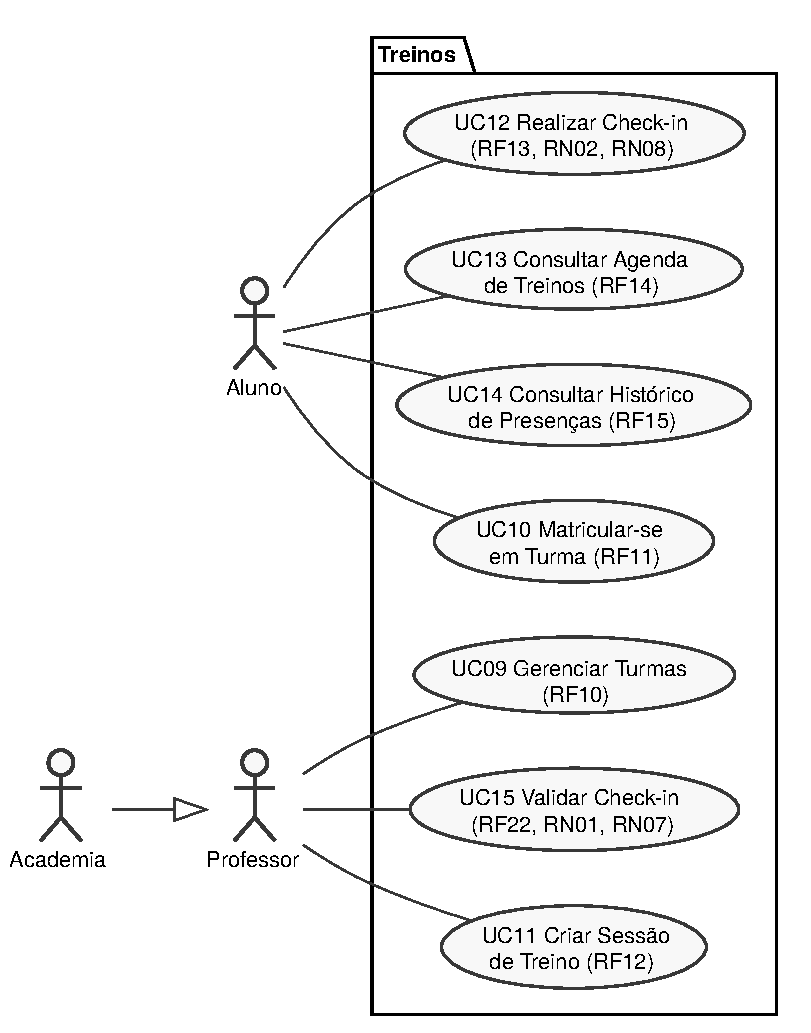
\includegraphics[width=0.62\textwidth]{figuras/uc-3-treinos.pdf}
  \fonte{Elaborado pelo autor (2026).}
\end{figure}

\begin{figure}[!htb]
  \centering
  \caption{Casos de uso do pacote Gamificação}
  \label{fig:uc-gamificacao}
  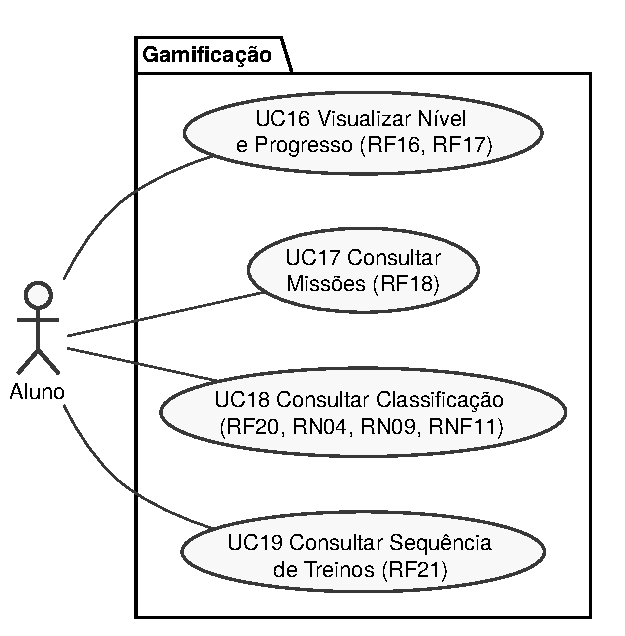
\includegraphics[width=0.5\textwidth]{figuras/uc-4-gamificacao.pdf}
  \fonte{Elaborado pelo autor (2026).}
\end{figure}

\begin{figure}[!htb]
  \centering
  \caption{Casos de uso do pacote Gestão}
  \label{fig:uc-gestao}
  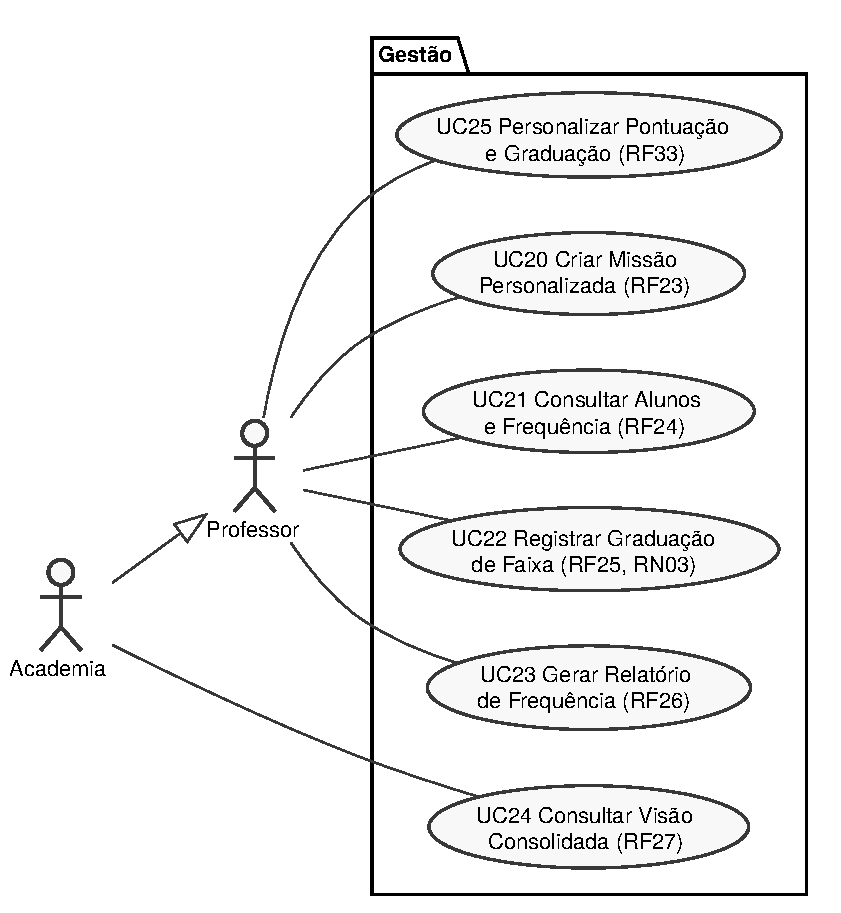
\includegraphics[width=0.62\textwidth]{figuras/uc-5-gestao.pdf}
  \fonte{Elaborado pelo autor (2026).}
\end{figure}

\begin{figure}[!htb]
  \centering
  \caption{Casos de uso do pacote Conformidade}
  \label{fig:uc-conformidade}
  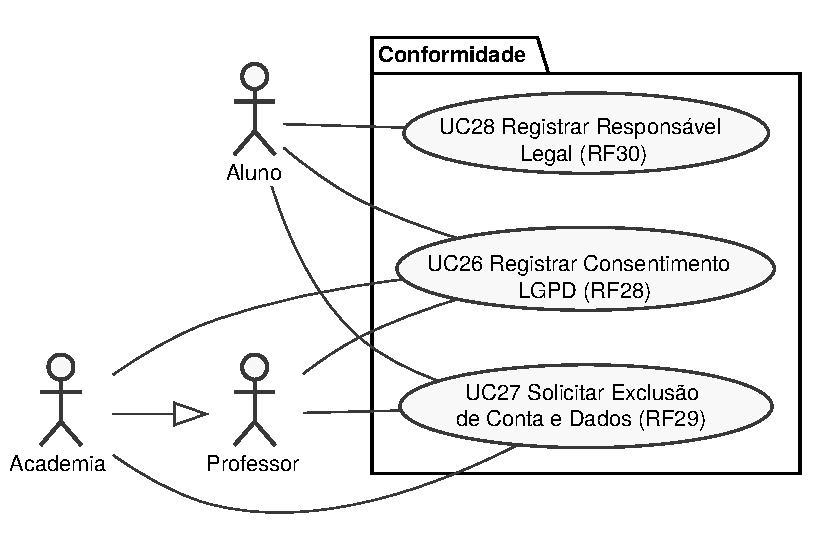
\includegraphics[width=0.62\textwidth]{figuras/uc-6-conformidade.pdf}
  \fonte{Elaborado pelo autor (2026).}
\end{figure}

\begin{figure}[!htb]
  \centering
  \caption{Casos de uso do pacote Retenção}
  \label{fig:uc-retencao}
  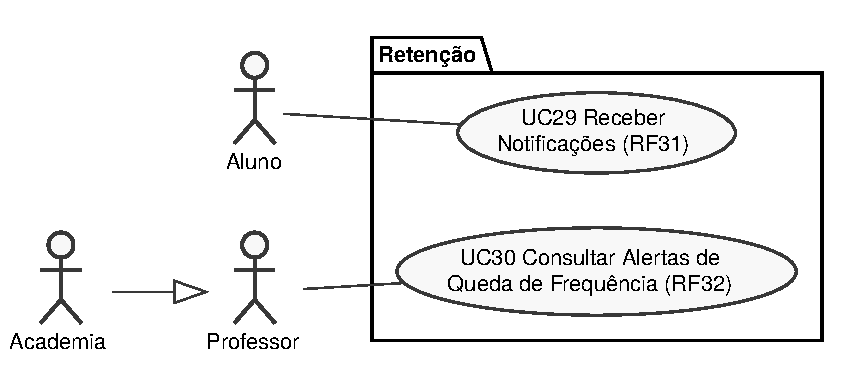
\includegraphics[width=0.62\textwidth]{figuras/uc-7-retencao.pdf}
  \fonte{Elaborado pelo autor (2026).}
\end{figure}

Cada caso de uso traz, no próprio diagrama, os requisitos que atende. A
especificação textual completa de cada um, com atores, pré-condições,
fluxos e pós-condições, está no repositório do projeto (\autoref{ap:artefatos}). A situação de
implementação de cada requisito está na
\autoref{sec:situacao-implementacao}.

\subsection{Descrição dos casos de uso principais}

O caso de uso central do aplicativo é o registro de presença (UC12),
porque dele derivam pontos, sequência, medalhas, missões e relatórios. O
\autoref{qua:uc12-uc15} descreve esse caso de uso e o que o completa, a
validação da presença (UC15), de acordo com o comportamento implementado.

\begin{quadro}[!htb]
  \caption{Descrição dos casos de uso UC12 e UC15}
  \label{qua:uc12-uc15}
  \centering
  \footnotesize
  \begin{tabular}{|p{2.7cm}|p{10.6cm}|}
    \hline
    \textbf{Caso de uso} & \textbf{UC12 -- Realizar \textit{check-in}} (ator: Aluno; RF13, RN02, RN08, RNF01) \\ \hline
    Pré-condições & Aluno autenticado, com vínculo ativo e matrícula ativa na turma da sessão. \\ \hline
    Fluxo principal & 1. O aluno abre a tela inicial, que destaca a próxima sessão. 2. O aluno toca em ``Fazer \textit{check-in}''. 3. O sistema verifica a sessão, a matrícula, a janela de tempo e a inexistência de \textit{check-in} anterior. 4. O sistema grava o \textit{check-in} com situação ``pendente'' e atualiza o botão. \\ \hline
    Fluxos alternativos & 3a. Janela ainda não aberta ou já encerrada: o sistema informa o motivo e não grava (RN08). 3b. \textit{Check-in} já existente: o sistema informa e não grava (RN02). 3c. Sessão cancelada ou aluno sem matrícula ativa: o sistema recusa. \\ \hline
    Pós-condição & \textit{Check-in} pendente de validação; nenhum ponto creditado ainda (RN01). \\ \hline\hline
    \textbf{Caso de uso} & \textbf{UC15 -- Validar \textit{check-in}} (ator: Professor, herdado pela Academia; RF22, RN01, RN07) \\ \hline
    Pré-condições & Existem \textit{check-ins} em sessões sob responsabilidade do gestor. \\ \hline
    Fluxo principal & 1. O gestor abre a chamada da sessão do dia. 2. O sistema lista os alunos matriculados e os \textit{check-ins} feitos. 3. O gestor confirma a presença de cada aluno que fez \textit{check-in}. 4. Ao confirmar, o sistema credita o XP no \textit{check-in} e na classificação do aluno, na mesma transação. \\ \hline
    Fluxos alternativos & 3a. O gestor desfaz uma confirmação: o \textit{check-in} volta a ``pendente'' e o sistema estorna os pontos. 3b. Aluno sem \textit{check-in}: aparece como ausente, e o gestor não pode registrar presença em nome dele. \\ \hline
    Pós-condição & Presença confirmada e pontuação atualizada, ou \textit{check-in} mantido como pendente. \\ \hline
  \end{tabular}
  \fonte{Elaborado pelo autor (2026).}
\end{quadro}

\section{Modelagem estática}
\label{sec:modelagem-estatica}

Como o Cloud Firestore é um banco de dados NoSQL orientado a documentos,
a modelagem estática é apresentada como um modelo de coleções, e não como
um diagrama de classes de um banco relacional. A \autoref{fig:modelo-dados}
mostra as coleções principais, seus campos mais relevantes e as relações
entre elas. Os identificadores de alguns documentos são
\textbf{determinísticos}, isto é, formados a partir de outros
identificadores: o \textit{check-in} tem identificador
\texttt{sessaoId\_alunoId}, o que garante por construção a regra RN02
(um \textit{check-in} por aluno por sessão); a matrícula usa
\texttt{turmaId\_alunoId}; o progresso de missão,
\texttt{missaoId\_alunoId}; e a classificação,
\texttt{alunoId\_responsavelId\_AAAA-MM}, que separa a pontuação por escopo
de vínculo (RN09) e por mês (RN04). A medalha usa o identificador do
marco (por exemplo, \texttt{treinos-10}), o que impede concedê-la duas
vezes ao mesmo aluno (RF19), e a estrutura de faixas usa o do
responsável, que tem uma única estrutura (RF33).

\begin{figure}[!htb]
  \centering
  \caption{Modelo de dados do RoundUp no Cloud Firestore}
  \label{fig:modelo-dados}
  \begin{tikzpicture}[
      font=\tiny,
      col/.style={draw, rectangle split, rectangle split parts=2, align=left,
                  text width=3.55cm, inner sep=2.5pt, rectangle split part fill={black!12,white}},
      rel/.style={thin}]
    \node[col, anchor=north] (usu) at (0,0) {\textbf{usuarios}
      \nodepart{second} id, nome\\ perfil: aluno $|$ professor $|$ academia\\ modalidades, faixaOuGrau\\ graduacoes (por modalidade)\\ faixasEstruturadas (por modalidade)\\ autonomo (só professor)\\ preferenciasNotificacao\\ participaClassificacao};
    \node[col, anchor=north] (vin) at (4.8,0) {\textbf{vinculos}
      \nodepart{second} id: solicitante\_destinatario\\ solicitanteId, destinatarioId\\ tipo (derivado dos perfis)\\ status: pendente $|$ aceito $|$\\ \quad recusado $|$ encerrado};
    \node[col, anchor=north] (tur) at (9.6,0) {\textbf{turmas}
      \nodepart{second} id, nome, modalidade, nivel\\ responsavelId, professorId\\ diasSemana, horários\\ ativa};
    \node[col, anchor=north] (chk) at (0,-4.3) {\textbf{checkins}
      \nodepart{second} id: sessao\_aluno\\ sessaoId, alunoId\\ responsavelId, dataHora\\ status: pendente $|$ validado $|$\\ \quad rejeitado\\ pontos, validadoPor\\ classificacaoId, professorId};
    \node[col, anchor=north] (ses) at (4.8,-4.3) {\textbf{sessoes}
      \nodepart{second} id, turmaId, responsavelId\\ inicio, fim\\ janelaCheckInInicio, janelaCheckInFim\\ status\\ leitoresIds[\,]};
    \node[col, anchor=north] (mat) at (9.6,-4.3) {\textbf{matriculas}
      \nodepart{second} id: turma\_aluno\\ turmaId, alunoId, responsavelId\\ professorId\\ status: ativa $|$ inativa};
    \node[col, anchor=north] (cla) at (0,-8.2) {\textbf{classificacoes}
      \nodepart{second} id: aluno\_responsavel\_AAAA-MM\\ alunoId, responsavelId\\ periodo, pontos\\ leitoresIds[\,], origemCheckinId};
    \node[col, anchor=north] (mis) at (4.8,-8.2) {\textbf{missoes} e \textbf{missoesProgresso}
      \nodepart{second} titulo, tipo, meta, pontos\\ responsavelId, ativa\\ publicoAlvo: todos $|$ turma $|$ alunos\\ turmaId, alunosAlvoIds[\,]\\ vigenciaInicio, vigenciaFim\\ leitoresIds[\,], situacao\\ id: missao\_aluno, progressoAtual\\ concluida, pontosCreditados};
    \node[col, anchor=north] (gra) at (9.6,-8.2) {\textbf{configuracoesGamificacao}
      \nodepart{second} id: responsavelId\\ pontosPorCheckin\\ pontosPorMissao, niveisXp};
        \node[col, anchor=north] (med) at (0,-12.6) {\textbf{usuarios/\{id\}/medalhas}
      \nodepart{second} id: marco (ex.: treinos-10)\\ tipo, quantidade, rotulo\\ conquistadaEm, origem\\ registradaEm};
    \node[col, anchor=north] (grd) at (4.8,-12.6) {\textbf{graduacoes}
      \nodepart{second} alunoId, responsavelId\\ modalidade, grau (texto)\\ faixaId, faixaNome, faixaCor\\ grauNumero, dataGraduacao};
    \node[col, anchor=north] (est) at (9.6,-12.6) {\textbf{estruturasFaixas}
      \nodepart{second} id: responsavelId\\ modalidades: mapa de\\ \quad modalidade $\rightarrow$ faixas[\,]\\ \quad (id, nome, cor, graus)};
    \draw[rel] (usu.east |- 0,-0.9) -- node[above]{1 : N} (vin.west |- 0,-0.9);
    \draw[rel] (vin.east |- 0,-0.9) -- node[above]{escopo} (tur.west |- 0,-0.9);
    \draw[rel] (tur.south) -- node[right]{1 : N} (mat.north);
    \draw[rel] (tur.south west) -- node[above, sloped]{1 : N} (ses.north east);
    \draw[rel] (ses.west |- 0,-5.2) -- node[above]{1 : N} (chk.east |- 0,-5.2);
    \draw[rel] (chk.south) -- node[right]{credita (RN01)} (cla.north);
        \draw[rel] (gra.west) -- node[above]{valores} (mis.east);
    \draw[rel] (est.west) -- node[above]{faixas} (grd.east);
  \end{tikzpicture}
  \fonte{Elaborado pelo autor (2026), a partir de \texttt{src/types/index.ts}.
         Omitidas da figura: \texttt{consentimentosLGPD}
         (registros imutáveis), \texttt{notificacoes} (registro de envios,
         escrito só pelas Cloud Functions) e os subdocumentos privados de
         \texttt{usuarios}, legíveis só pelo dono: \texttt{privado/dados}
         (e-mail, data de nascimento e responsável legal, RNF04),
         \texttt{privado/vinculos} e \texttt{privado/notificacoes}.}
\end{figure}

Duas decisões de modelagem merecem destaque, porque nasceram de
limitações do motor de regras do Firestore descobertas durante os testes
automatizados (\autoref{sec:testes-prototipo}):

\begin{itemize}
  \item \textbf{Lista de leitores na sessão.} O Firestore só autoriza uma
        consulta de lista quando consegue provar, pelo formato do filtro,
        que todos os documentos retornáveis são permitidos. Uma regra do
        tipo ``o aluno está matriculado na turma desta sessão'' exigiria
        consultar outra coleção e não pode ser usada em listas. Por isso,
        cada sessão guarda um campo \texttt{leitoresIds} com o responsável,
        o professor e os alunos matriculados, e a regra de leitura apenas
        verifica se o usuário está nessa lista. A manutenção da lista,
        quando uma matrícula é criada, cancelada ou reativada, é feita por
        Cloud Functions. O mesmo padrão foi usado na classificação: cada
        documento guarda os alunos do mesmo escopo que participam do
        \textit{ranking}, e quem desativa a participação (RNF11) sai das
        listas dos colegas. Nas missões, a lista de leitores reflete o
        público-alvo e a vigência (RF23); como a regra de uma consulta de
        lista também não consegue comparar a vigência com a hora atual,
        uma Cloud Function agendada atualiza essa lista todos os dias, às
        00h05.
  \item \textbf{Vínculos em documento privado.} Para que as regras possam
        verificar se um aluno tem vínculo ativo com um responsável sem
        expor o grafo de vínculos a todos os usuários, essa informação foi
        movida para um subdocumento privado de cada usuário
        (\texttt{usuarios/\{uid\}/privado/vinculos}), legível pelas regras,
        mas fechado para os demais clientes (RNF04).
\end{itemize}

\section{Modelagem dinâmica}
\label{sec:modelagem-dinamica}

A \autoref{fig:sequencia-checkin} apresenta o diagrama de sequência do
ciclo completo de uma presença: o aluno registra o \textit{check-in}
(UC12), o professor o valida (UC15) e o sistema credita os pontos. Como
os pontos só existem depois da validação (RN01), o aluno não consegue
acumular XP sem ter, de fato, comparecido ao treino.

\begin{figure}[!htb]
  \centering
  \caption{Diagrama de sequência do registro e da validação de presença}
  \label{fig:sequencia-checkin}
  \begin{tikzpicture}[font=\scriptsize,
      obj/.style={draw, minimum width=2.3cm, minimum height=0.6cm, fill=black!8},
      msg/.style={-{Stealth[length=2mm]}},
      ret/.style={-{Stealth[length=2mm]}, dashed}]
    \node[obj] (a) at (0,0) {Aluno (app)};
    \node[obj] (c) at (3.6,0) {Serviço de check-in};
    \node[obj] (f) at (7.2,0) {Firestore};
    \node[obj] (p) at (10.8,0) {Professor (app)};
    \foreach \n in {a,c,f,p} \draw[dotted] (\n.south) -- ++(0,-9.0);
    \draw[msg] (0,-0.8) -- node[above]{realizarCheckIn(sessao)} (3.6,-0.8);
    \draw[msg] (3.6,-1.4) -- node[above]{transação: ler sessão e matrícula} (7.2,-1.4);
    \draw[ret] (7.2,-2.0) -- node[above]{dados} (3.6,-2.0);
    \node[draw, fill=white, align=left, text width=3.4cm, font=\tiny, anchor=west] at (3.75,-2.6) {verifica janela (RN08), matrícula ativa e duplicidade (RN02)};
    \draw[msg] (3.6,-3.95) -- node[above]{gravar check-in ``pendente''} (7.2,-3.95);
    \draw[ret] (3.6,-4.5) -- node[above]{confirmação} (0,-4.5);
    \draw[msg] (10.8,-5.2) -- node[above]{listar check-ins da sessão} (7.2,-5.2);
    \draw[msg] (10.8,-5.9) -- node[above]{validarCheckIn(id, ``validado'')} (3.6,-5.9);
    \draw[msg] (3.6,-6.6) -- node[above]{transação: check-in.pontos = valor configurado} (7.2,-6.6);
    \draw[msg] (3.6,-7.2) -- node[above]{classificação do mês += pontos (RN01)} (7.2,-7.2);
    \draw[ret] (3.6,-7.8) -- node[above]{validado} (10.8,-7.8);
    \draw[ret] (7.2,-8.6) -- node[above]{novo XP, nível, sequência e medalhas} (0,-8.6);
  \end{tikzpicture}
  \fonte{Elaborado pelo autor (2026).}
\end{figure}

O nível e a sequência não são gravados no banco: eles são calculados no
aplicativo, a cada carregamento, a partir dos \textit{check-ins} validados
e da pontuação acumulada, o que evita manter dados derivados
sincronizados. As medalhas seguem outro caminho: são gravadas por uma
Cloud Function no momento em que o marco é atingido, para registrar a data
da conquista (RF19), e não são retiradas se a contagem cair depois.

